\begin{appendices}
	\chapter{Figures}
	\begin{figure}[h]
		\centering
		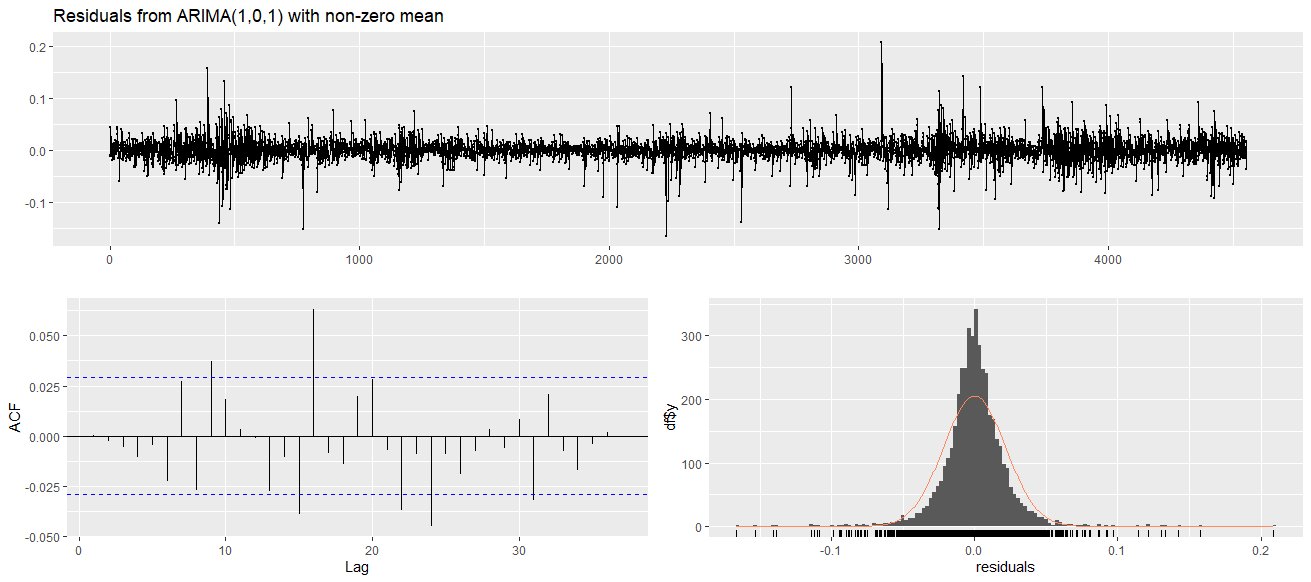
\includegraphics[width=0.7\linewidth]{content/plots/residual_plot_1_1.png}
		\caption{Residual Plots for the ARIMA(1,0,1) model for the Log Prices}
		\label{fig:residual_plot_1_1}
	\end{figure}
	
	\begin{figure}[!h]
		\centering
		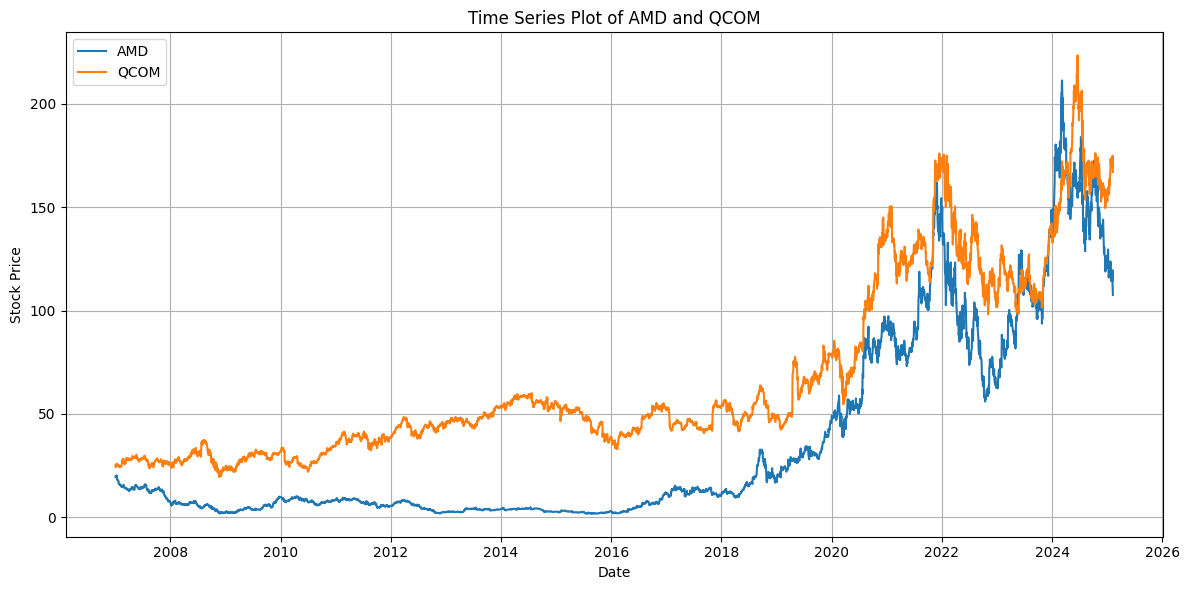
\includegraphics[width=0.8\linewidth]{content/plots/QCOM_AMD.png}
		\caption{Cumulative Returns of QCOM and AMD}
		\label{fig:amd_qcom_cumul_returns}
	\end{figure}
	
		\begin{figure}[!h]
		\centering
		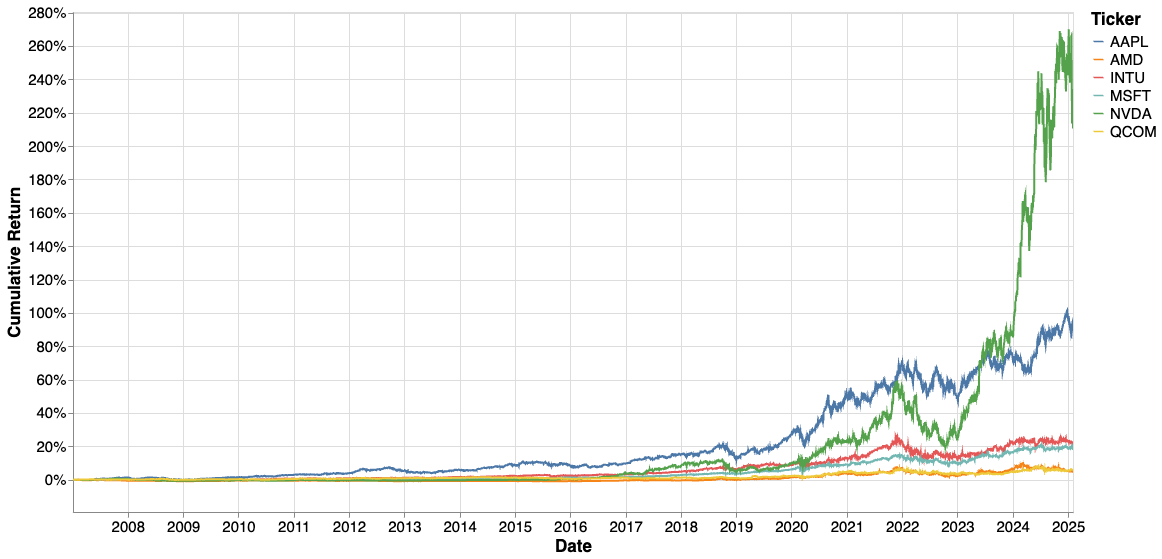
\includegraphics[width=0.8\linewidth]{content/plots/visualization.png}
		\caption{Cumulative Returns of QCOM and AMD}
		\label{fig:sample_securities}
	\end{figure}
	
	\chapter{Tables}
	
	\begin{table}[!h]
		\centering
		\caption{Ljung-Box Test Model Fit}
		\begin{tabular}[t]{lccccc}
			\toprule
			   & Method &Lag order& t-statistic & $p$-value & Outcome  \\
			\midrule
			ARCH & Standard Residuals & 10 & 4.5922 & 0.9167 & No autocorrelation  \\				
			GARCH & Squared Residuals & 10& 9.6976 & 0.4674 & Stationary  \\				
			\bottomrule
		\end{tabular}\label{tab:ARCH_GARCH}
	\end{table}
	
	\begin{table}[!h]
		\centering
		\caption{Information Criteria for GARCH-type Models}
		\begin{tabular}{lcccc}
			\toprule
			\textbf{Model} & \textbf{Akaike} & \textbf{Bayes} & \textbf{Shibata} & \textbf{Hannan-Quinn} \\
			\midrule
			GARCH(1,1)     & -2.020259 & -1.896058 & -2.022828 & -1.970093 \\
			EGARCH         & \textcolor{red}{-2.064928} & -1.909676 & -2.068896 & -2.002220 \\
			GJR-GARCH      & -2.049684 & -1.894432 & -2.053652 & -1.986976 \\
			IGARCH         & -2.024722 & -1.916046 & -2.026700 & -1.980826 \\
			TGARCH         & -2.045296 & -1.905569 & -2.048528 & -1.988858 \\
			\bottomrule
		\end{tabular}\label{tab:GARCH_model}
	\end{table}
	

\end{appendices}